\documentclass{../c-lecture}

\subtitle{Calculation}

\begin{document}

\begin{frame}
  \titlepage{}
\end{frame}
\begin{frame}
  \frametitle{Outline}
  \tableofcontents{}
\end{frame}

\section{Basic mathematic operations in C}

\begin{frame}
  \frametitle{Basic operations}
  \begin{table}
  \begin{tabular}{cc}
    \toprule

    Addition &
    $+$\\

    \midrule

    Subtraction &
    $-$\\

    \midrule

    Division &
    $/$\\

    \midrule

    Multiplication &
    $*$\\

    \midrule

    Modulus &
    $\%$\\

    \bottomrule
  \end{tabular}
  \end{table}
\end{frame}

\begin{frame}
  \frametitle{Modulo}
  \begin{itemize}
    \item Only can be used by \textbf{\color{Orange} int} operands
    \begin{itemize}
      \item $5 \% 4 = 1$
      \item $7 \% 88 = 7$
      \item $-20 \% 7 = -6$
      \item $20 \% -7 = 6$
      \item $-20 \% -7 = -6$
    \end{itemize}
  \end{itemize}
\end{frame}

\begin{frame}[fragile]
  \frametitle{Mean of 3 Numbers}
  \begin{minted}[bgcolor=Black]{c}
#include <stdio.h>
int main(void) {
  float num1, num2, num3, sum, average;
  printf("Enter 3 number: \n");
  scanf("%f",&num1);
  scanf("%f",&num2);
  scanf("%f",&num3);
  sum = num1 + num2 + num3;
  average = sum / 3;
  printf("mean = ");
  printf("%f\n", average);
  return 0;
}
  \end{minted}
\end{frame}

\section{Effect of type and type conversion}

\begin{frame}
  \frametitle{General rules of type conversion}
  \begin{itemize}
    \item
      If either operand is \textit{\color{Orange} long double},
      convert the other to \textit{\color{Orange} long double}.

    \item
      Otherwise, if either operand is \textit{\color{LimeGreen} double},
      convert the other to \textit{\color{LimeGreen} double}.

    \item
      Otherwise, if either operand is \textit{\color{Cyan} float},
      convert the other to \textit{\color{Cyan} float}.

    \item
      Otherwise, convert \textit{\color{Orange} char} and
      \textit{\color{Orange} short} to
      \textit{\color{Orange} int}.

    \item
      Then, if either operand is \textit{\color{LimeGreen} long}, convert
      the other to \textit{\color{LimeGreen} long}.
  \end{itemize}
\end{frame}

\begin{frame}
  \frametitle{Effect of types}
  \begin{itemize}
    \item Type of operands determines the type of the result
    \begin{itemize}
      \item The type of output is the type of operands (after conversion)
    \end{itemize}
    \item int <op> int $\Rightarrow$ int
    \item int <op> long $\Rightarrow$ long
    \item float <op> float $\Rightarrow$ float
    \item float <op> int $\Rightarrow$ float
    \item double <op> float $\Rightarrow$ double
  \end{itemize}
\end{frame}

\begin{frame}
  \frametitle{Effect of types}
  \begin{itemize}
    \item
      If both operand of division ($/$) is \textit{\color{Orange} int}
    \item \textrightarrow\ data lost
  \end{itemize}
\end{frame}

\begin{frame}
  \frametitle{Effect of types \& Explicit casts}
  \begin{table}
  \begin{tabular}{ccc}
    \toprule

    Expression &
    Result &
    Type of result \\

    \midrule

    $(double) 1 + 2.0f$ &
    $3.0$ &
    $double$ \\

    \midrule

    $(int) 2.69 + 4$ &
    $6$ &
    $int$ \\

    \midrule

    $(double) 1 / 2$ &
    $0.5$ &
    $double$ \\

    \midrule

    $1 / (int) 2.0$ &
    $0$ &
    $int$ \\

    \midrule

    $(double) (1 / 2)$ &
    $0.0$ &
    $double$ \\

    \midrule

    $(int)((double) 1 / 2)$ &
    $0$ &
    $int$ \\

    \bottomrule
  \end{tabular}
  \end{table}
\end{frame}

\section{Precedence}

\begin{frame}
  \frametitle{Precedence}
  \begin{enumerate}
    \item Parenthesis
    \item Unary $+$ $-$ (for sign): $+4$, $-8$
    \item Explicit casting
    \item $/$ $*$ $\%$
    \item Binary $+$ $-$: $4 + 8$
    \item If multiple $+$ $-$ or $/$ $*$ $\%$: from left to right
  \end{enumerate}
\end{frame}

\begin{frame}[fragile]
  \begin{minted}[bgcolor=Black]{c}
#include <stdio.h>

int main(void){
  double num1, num2;
  int sum;
  printf("Enter 2 number: \n");
  scanf("%lf", &num1);
  scanf("%lf", &num2);
  sum = (int)num1 + (int)num2;
  printf("%d\n", sum);
  return 0;
}
  \end{minted}
\end{frame}

\begin{frame}[fragile]
  \begin{minted}[bgcolor=Black]{c}
#include <stdio.h>

int main(void){
  double num1, num2, fpart1, fpart2, sum;
  printf("Enter 2 number: \n");
  scanf("%lf", &num1);
  scanf("%lf", &num2);
  fpart1 = num1 - (int)num1;
  fpart2 = num2 - (int)num2;
  sum = fpart1 + fpart2;
  printf("%lf\n", sum);
  return 0;
}
  \end{minted}
\end{frame}

\section{Advanced mathematical operations}

\begin{frame}[fragile]
  \frametitle{Increment \& Decrement of Variables}
  \begin{itemize}
    \item Unary operators only for variables
    \item $++$: increase by one
    \item $--$: decrease by one
  \end{itemize}
  \begin{minted}[bgcolor=Black]{c}
int i = 10;
i = i + 1; // i = 11
i++;       // i = 12
++i;       // i = 13
i--;       // i = 12
--i;       // i = 11
i = i - 1; // i = 10
  \end{minted}
\end{frame}

\begin{frame}[fragile]
  \frametitle{Increment \& Decrement (cont’d)}
  \begin{itemize}
    \item
      {\color{Cyan} Postfix:} Use the value then apply the
      operator
    \item
      {\color{Cyan} Prefix:} Apply the operator then use the value
  \end{itemize}
  \begin{minted}[bgcolor=Black]{c}
int i = 10, k = 6, j;
j = i + 1;  // i = 10, j = 11
j = i++;    // i = 11, j = 10
j = ++i;    // i = 12, j = 12
j = i--;    // i = 11, j = 12
j = --i;    // i = 10, j = 10
j = i - 1;  // i = 10, j = 9
  \end{minted}
\end{frame}

\begin{frame}[fragile]
  \frametitle{Assignment Combined with Operation}
  \begin{itemize}
    \item These are equal
    \begin{itemize}
      \item <variable> <op> = <expression>;
      \item
        <variable> = <variable> <op> (<expression>)
    \end{itemize}
  \end{itemize}
  \begin{minted}[bgcolor=Black]{c}
int i = 9, j = 20;
i += 1; // i = i + 1; i = 10
j /= i; // j = j / i; j = 2
i *= i + j - 6 + i / j;
/*i = i * (i + j - 6 + (i / j)); i = 110*/
  \end{minted}
\end{frame}

\begin{frame}[fragile]
  \frametitle{Multiple assignment}
  \begin{itemize}
    \item More than one assignment in a statement
    \begin{itemize}
      \item From right to left
    \end{itemize}
  \end{itemize}
  \scriptsize
  \begin{minted}[bgcolor=Black]{c}
int i, j, k, l;
i = j = k = l = 1;
i += j *= --k -= 3 / l;
// step 1
i += j *= --k -= 3
// step 2
i += j *= --(k -= 3) // [k = -2]
// step 3
i += j *= --k // [k = -3]
// step 3
i += j *= -3 // [j = -3]
// step 4
i += -3 // [i = -2]
// result
// i = -2, j = -3, k = -3, l = 1
  \end{minted}
\end{frame}

\begin{frame}
  \frametitle{Precedence}
  \begin{table}
  \begin{tabular}{cc}
    \toprule

    Operator &
    Direction \\

    \midrule

    $( )$&
    \\

    \midrule

    $++$ $--$ $(type)$ &
    \\

    \midrule

    $*$ $/$ $\%$ &
    Left to Right \\

    \midrule

    $+$ $-$ &
    Left to Right \\

    \midrule

    $+=$ $-=$ $*=$ $/=$ $\%=$ &
    Right to Left \\

    \bottomrule
  \end{tabular}
  \end{table}
\end{frame}

\begin{frame}[fragile]
  \frametitle{Arithmetic on characters}
  \begin{itemize}
    \item \mintinline{c}|char| can be used as 8-bit integer
    \item All arithmetic operation can be used with characters
  \end{itemize}
  \begin{minted}[bgcolor=Black]{c}
/* A: 65, B: 66, C: 67, … */
char c = 'A', ch;
int i;
c++; // c = 66, c = 'B'
ch = c;
ch += 3; // ch = 69, ch = 'E'
i = c - ch + 'X' - 'Z'; // i = -5
  \end{minted}
\end{frame}

\begin{frame}
  \frametitle{sizeof operator}
  \begin{itemize}
    \item \mintinline{c}|sizeof| is a unary operator
    \begin{itemize}
      \item Return the size of operand in bytes
      \item Operand can be {\color{Cyan} Variable, value or type}
      \item The operand inside the \mintinline{c}|sizeof()| operator is not evaluated
    \end{itemize}
  \end{itemize}
\end{frame}

\begin{frame}[fragile]
  \frametitle{sizeof operator}
  \begin{minted}[bgcolor=Black]{c}
int size, i = 10;
size = sizeof i;     // 4
size = sizeof(i);    // 4
size = sizeof(2000); // 4
size = sizeof(char); // 1
  \end{minted}
\end{frame}

\begin{frame}
  \frametitle{Precedence}
  \begin{table}
  \begin{tabular}{cc}
    \toprule

    Operator &
    Direction \\

    \midrule

    $( )$&
    \\

    \midrule

    $++$ $--$ $(type)$ $sizeof()$ &
    \\

    \midrule

    $*$ $/$ $\%$ &
    Left to Right \\

    \midrule

    $+$ $-$ &
    Left to Right \\

    \midrule

    $+=$ $-=$ $*=$ $/=$ $\%=$ &
    Right to Left \\

    \bottomrule
  \end{tabular}
  \end{table}
\end{frame}

\begin{frame}[fragile]
  \frametitle{Undefined Statements}
  \begin{itemize}
    \item
      When standard does \textbf{\color{RubineRed} not} tell what will
      happen
    \item Examples
  \end{itemize}
  \begin{minted}[bgcolor=Black]{c}
int i, j, k;

k = i = 10;
j = i++ + k + --i; // j = 29 or 30?

i = j = 10;
i = j + i++; // i = 11 or ???
  \end{minted}
\end{frame}

\begin{frame}
  \frametitle{Overflow and Underflow}
  \begin{itemize}
    \item Computer's precision is limited
    \begin{itemize}
      \item
        {\color{Orange} The number of bits} in each type is
        limited
      \item double [-1e308, 1e308]
    \end{itemize}
    \item Overflow
    \begin{itemize}
      \item When result is larger than specified ranges
      \item 1e300 * 1e200
    \end{itemize}
    \item Underflow
    \begin{itemize}
      \item When the result is too smaller than precision
      \item 1e-300 * 1e-200
    \end{itemize}
  \end{itemize}
\end{frame}

\begin{frame}[fragile]
  \frametitle{Quadratic Term}
  \begin{minted}[bgcolor=Black]{c}
#include <stdio.h>

int main(void){
  double a, b, c, x, result;
  printf("Enter a, b, c, x: ");
  scanf("%lf", &a);
  scanf("%lf", &b);
  scanf("%lf", &c);
  scanf("%lf", &x);
  result = a * x * x + b * x + c;
  printf("%lf\n", result);
  return 0;
}
  \end{minted}
\end{frame}

\section{Mathematic library}

\begin{frame}[fragile]
  \frametitle{Math library}
  \begin{itemize}
    \item \mint{c}|#include <math.h>|
  \end{itemize}
  \scriptsize
  \begin{minted}[bgcolor=Black]{c}
double f = 36;
fabs(-f) // 36.000000
sqrt(f) // 6.00000
pow(f, 0.5) // 6.000000
ceil(-10.2) // -10.000000
ceil(10.2) // 11.000000
floor(-10.2) // -11.000000
floor(10.2) // 10.000000
fmax(10.1, 20.2) // 20.2
fmin(10.1, 20.2) // 10.1
rint(10.2) // 10.0
rint(-10.2) // -10.0
rint(20.6) // 21.0
rint(-20.6) // -21.0
  \end{minted}
\end{frame}

\begin{frame}[fragile]
  \frametitle{Math library}
  \begin{minted}[bgcolor=Black]{c}
const double PI = 3.141592653589793;
const double E = 2.7182818284590451;

// M_PI, M_E are defined in math.h

sin(PI) // 0.000000
cos(PI/2) // 0.000000
acos(1) // 0.000000
log(E)  // 1.000000
log(10) // 2.30258
exp(1) // 2.718282
  \end{minted}
\end{frame}

\begin{frame}[fragile]
  \frametitle{Perimeter and Area of Circle}
  \begin{minted}[bgcolor=Black]{c}
#include <stdio.h>
#include <math.h>

int main(void){
  double r;
  printf("Enter Radius");
  scanf("%lf", &r);
  double area = M_PI * pow(r, 2);
  double perimeter = 2 * M_PI * r;
  printf("Area = %lf\n", area);
  printf("Perimeter = %lf\n", perimeter);
  return 0;
}
  \end{minted}
\end{frame}

\section{Random Numbers}

\begin{frame}[fragile]
  \frametitle{Random Numbers}
  \begin{itemize}
    \item \mint{c}|#include <stdlib.h>|
    \item \mint{c}|rand()|
    \begin{itemize}
      \item A random number in $[0, RAND\_MAX]$
    \end{itemize}
    \item How does it work
    \begin{itemize}
      \item Start from a {\color{Orange} seed\_number}
      \item $X_0 = F(seed\_number)$
      \item $X_{n + 1} = F(X_n)$
    \end{itemize}
    \item Same seed
    \begin{itemize}
      \item Same random number sequence
    \end{itemize}
  \end{itemize}
\end{frame}

\begin{frame}[fragile]
  \frametitle{Random Numbers}
  \begin{itemize}
    \item We usually want different random number
    \begin{itemize}
      \item Run 1: 10, 20, 17, 1000, 23, 345, 30
      \item Run 2: 23, 904, 23, 346, 85, 234, 63
    \end{itemize}
    \item We should use different seed in each run
    \begin{itemize}
      \item How?
      \item Initialize seed by system time
    \end{itemize}
  \end{itemize}
  \begin{minted}[bgcolor=Black]{c}
#include <time.h>
time_t t = time(NULL);
srand(t);
  \end{minted}
\end{frame}

\begin{frame}[fragile]
  \frametitle{Random Numbers}
  \scriptsize
  \begin{minted}[bgcolor=Black]{c}
#include <stdio.h>
#include <stdlib.h>
#include <time.h>

int main(void) {
  int r1, r2;
  srand(0);
  r1 = rand();
  printf("r1 = %d\n", r1);
  time_t t = time(NULL);
  srand(t);
  r2 = rand();
  printf("r2 = %d\n", r2);
  return 0;
}
  \end{minted}
\end{frame}

\begin{frame}
  \frametitle{Random Numbers}
  \begin{itemize}
    \item First Run
    \begin{itemize}
      \item r1 = 38
      \item r2 = 1873
    \end{itemize}
    \item Second Run
    \begin{itemize}
      \item r1 = 38
      \item r2 = 1866
    \end{itemize}
    \item Third Run
    \begin{itemize}
      \item r1 = 38
      \item r2 = 1860
    \end{itemize}
  \end{itemize}
\end{frame}

\section{Type-generic math}

\begin{frame}
  \frametitle{\textit{tgmath.h}}
  \begin{itemize}
    \item The header \textit{\color{Orange} <tgmath.h>} includes the headers \textit{\color{LimeGreen} <math.h>} and \textit{\color{LimeGreen} <complex.h>}
      and defines several type-generic macros that determine which real or, when applicable, complex function to call based on the types of the arguments.
    \item Each of the arguments provided for these generic parameters that is of an integer type is casted to a double;
      Arguments of floating-point types are used without transformation (directly as float, double or long double).
    \item real function:
    \begin{itemize}
      \item \textit{float} variant XXXf
      \item \textit{double} variant XXX
      \item \textit{long double} variant XXXl
    \end{itemize}
  \end{itemize}
\end{frame}

\begin{frame}
  \frametitle{fabs}
  \begin{itemize}
    \item fabsf --- float
    \item fabs --- double
    \item fabsl --- long double
  \end{itemize}
\end{frame}

\begin{frame}
  \frametitle{Legends}
  \begin{figure}
    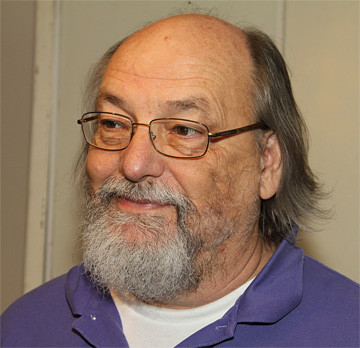
\includegraphics[height=.75\textheight]{./img/ken.jpg}
  \end{figure}
  \pause%
  \centering
  \color{Violet} Ken Thompson
\end{frame}

\begin{frame}
  \frametitle{Legends}
  \begin{itemize}
    \item he designed and implemented the original Unix operating system.
    \item he worked at Google, where he co-developed the Go programming language.
    \item he worked on regular expressions and early computer text editors QED and ed.
  \end{itemize}
\end{frame}

\end{document}
